% !TEX root = marvin.tex
% \vspace{-0.2in}
\section{Introduction}
\label{intro}


As robots become ubiquitous, one of the fundamental problems is to be able to route a fleet or swarm
of robots to perform a task. Several approaches have been developed to try to solve this task.
The traveling salesman problem (TSP) is a classic NP-Hard~\cite{vrp} problem in computer science, wherein 
an agent must visit a set of points while traveling the shortest possible distance.
The natural multi-agent generalization of this problem is known as the vehicle routing
problem (VRP)~\cite{vrp}, where multiple agents work in tandem to ensure that all points are visited exactly once.
% The vehicle routing problem~\citep{vrp} (VRP) is a multi-agent generalization to the well-known
% traveling salesman problem (TSP). \raquel{Ill first define TST and then VRP, as you did in the talk}
% Looking for the optimal routes for a fleet of vehicles to traverse
% a set of destinations, VRP has been shown to be NP-Hard~\citep{vrp}.
Despite a plethora of classic
approaches to these problems~\cite{concorde,lkh3}, solvers are typically structured for offline
planning and generally are unable to adapt their solutions online. Furthermore, these solvers do not
incorporate  online communication between the agents which is very desirable in many
practical settings. These are not necessarily weaknesses of the solutions but rather the
oversimplification of the problem definition itself.

Recently proposed deep learning methods have presented promising results in approximating solutions
with much faster runtime~\cite{pointer,combinatorialgraph,am,ean}. However, they are often tested on
simplistic planar graph benchmarks with limited exploration on multi-agent settings. Moreover, none
of these methods were designed towards dynamic environments where online communication can be very
beneficial.

% !TEX root = marvin.tex
\begin{figure}[t]
\begin{center}
\iflatexml
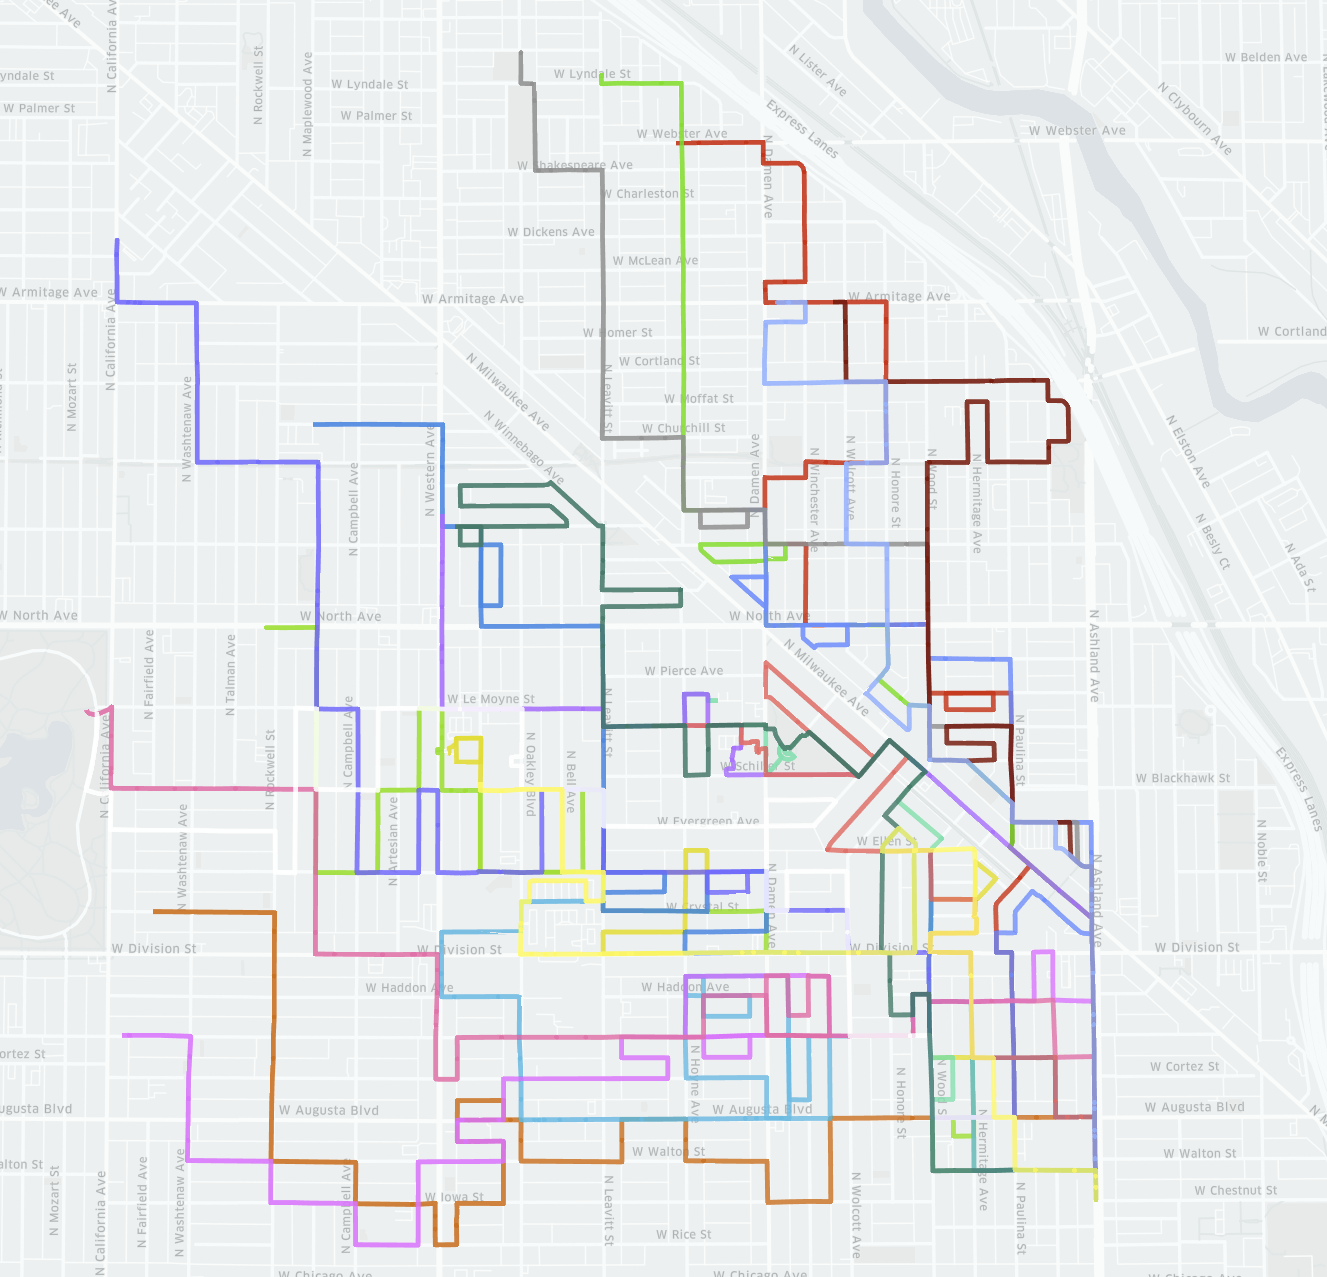
\includegraphics[width=6\textwidth,trim={3cm 0 6cm 10cm},clip]{figs/teaser.png}
\else
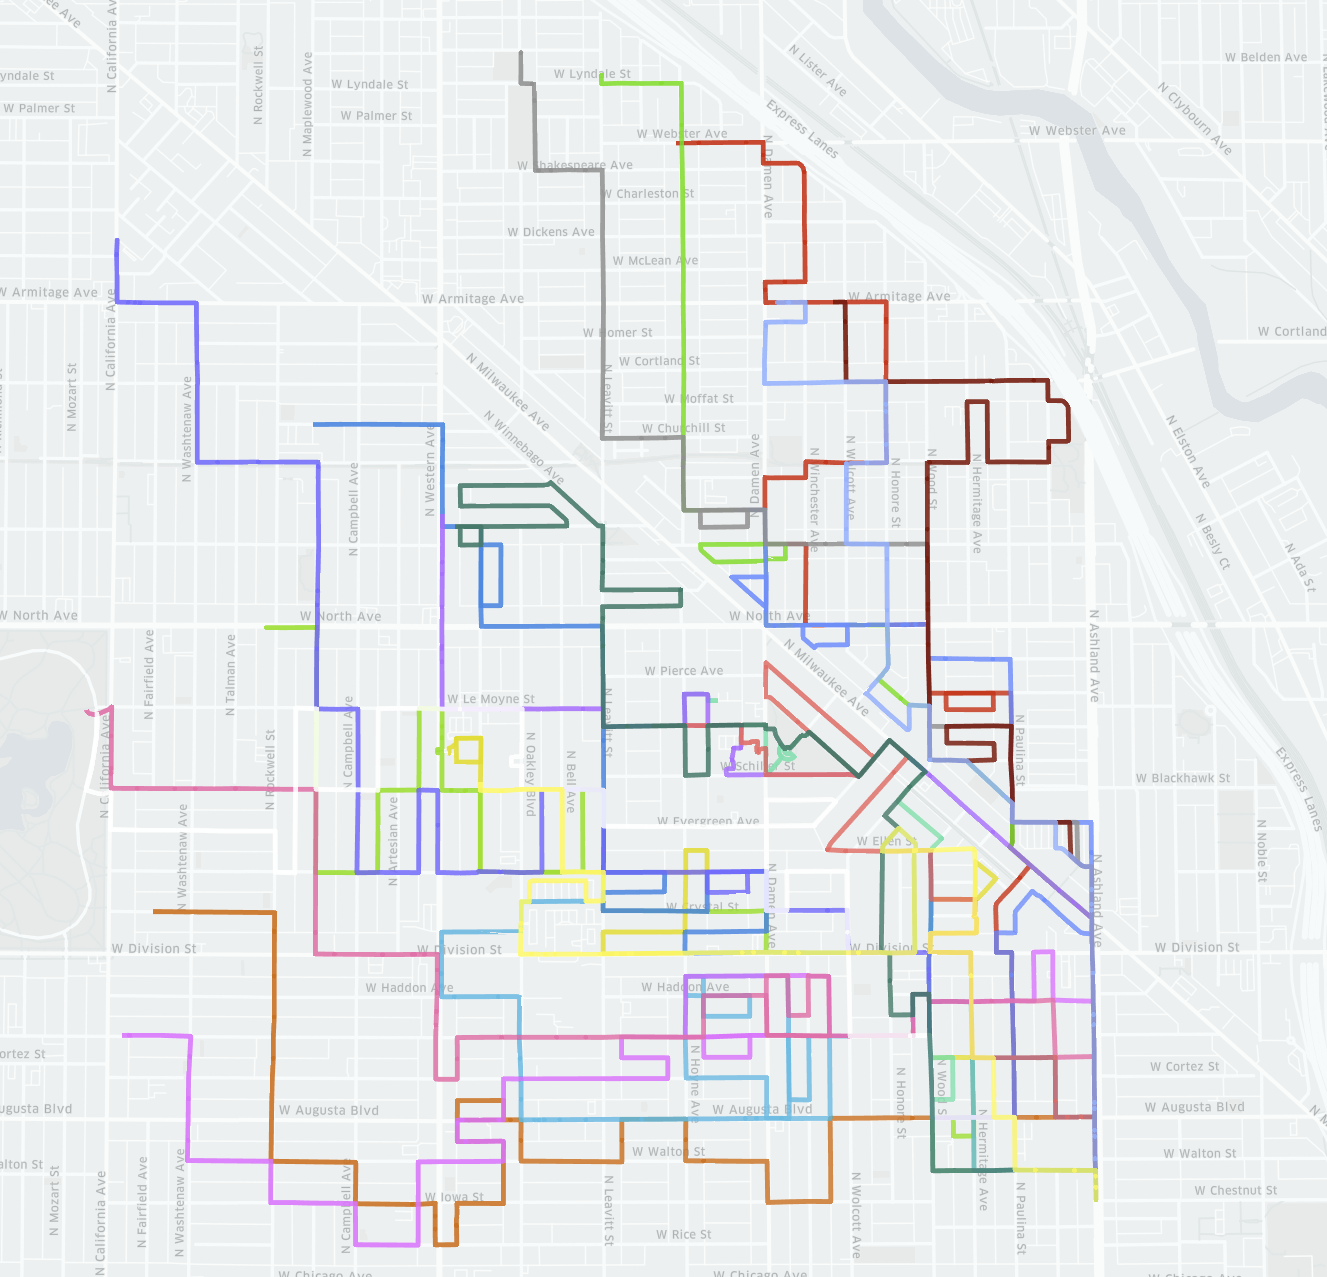
\includegraphics[width=0.94\columnwidth,trim={3cm 0 6cm 10cm},clip]{figs/teaser.png}
\fi
\vspace{-0.15in}
\caption{A visualization of the route produced by a fleet of twenty vehicles using our proposed
algorithm. Colors denote different vehicle trajectories.}
\label{fig:teaser}
\end{center}
\vspace{-0.25in}
\end{figure}
We focus on the realistic {\it multi-agent autonomous mapping problem}: given a fleet
of vehicles, find the minimum total cost to map an urban region subject to traffic conditions,
such that each road in the city is traversed at least a certain number of times, where the number is
unknown a priori. This is a realistic setting for autonomous mapping as a region might need to be
recollected due to  occlusions, heavy traffic, bad localization, sensor failure, bad weather
conditions, etc. Unfortunately neither VRP solutions nor existing deep learning methods perform well
in this difficult scenario.

In this paper we propose the Multi Agent Routing Value Iteration Network (MARVIN), a distributed
deep neural net tasked with the coordination of a swarm of vehicles to achieve a specific goal. In
particular, each agent performs local planning in a learned value iteration module which exploits
inter-agent communication through a novel learned communication protocol using the an attention mechanism.
As we focus on sparse road graphs, our second contribution is the  use of a dense
adjacency matrix that encodes pairwise edge information to speed up information exchange and enable
more rich node encodings.

We demonstrate the effectiveness of our approach on real road maps extracted from 18 different
cities from around the world, using realistic traffic flow
simulation~\citep{macroscopicsim,continuum}.
To create our training and evaluation examples containing the
aforementioned realistic mapping challenges, we randomly subsample subgraphs  on those cities, for
%We randomly subsample subgraphs for training and evaluation, and
each node in each graph we then randomly sample the number of times it has to be covered. Note that this information will be unknown to the fleet, and will only discovered upon reaching this number.
We exploit total traversal time as our primary evaluation metric, and show that
%and show that our approach outperforms
%state-of-the-art conventional VRP solver~\citep{lkh3}, as well as recently proposed deep learning
%models~\citep{am, ean, gvin}.
%The performance of our model is compared against a
%state-of-the-art conventional VRP solver~\citep{lkh3}, as well as recently proposed deep learning
%models~\citep{am, ean, gvin}, using total traversal time as our primary evaluation metric.
%Ultimately, we find that not only is
our approach achieves better performance than state-of-the-art conventional VRP solvers~\citep{lkh3}, as well as recently proposed deep learning
models~\citep{am, ean, gvin}. Furthermore, MARVIN
generalizing well  to the graph size and the number of agents guaranteeing a full
graph completion.
